\ifuniversity
\chapter*{ΣΥΝΟΠΤΙΚΗ ΠΑΡΟΥΣΙΑΣΗ ΤΗΣ ΔΙΔΑΚΤΟΡΙΚΗΣ ΔΙΑΤΡΙΒΗΣ}
\thispagestyle{empty}

Τα αποκεντρωμένα συστήματα βασισμένα στις αλυσίδες απόδειξης εργασίας ή μεριδίου
αναπτύσσονται ραγδιαία από το ντεμπούτο τους μέσω του Bitcoin το 2008 μέχρι σήμερα.
Η ανάπτυξη αυτή έχει οδηγήσει σε δύο κεντρικά προβλήματα στην περιοχή. Από τη μία,
τα συστήματα αλυσίδων που επιβιώνουν μακροχρόνια διατηρούν, αποθηκεύουν και αναμεταδίδουν
στο δίκτυο ολοένα και μακρύτερες αλυσίδες. Ιδιαίτερα σε νεότερα συστήματα όπως το Ethereum
όπου τα blocks των αλυσίδων παράγονται με ταχύτερο ρυθμό αλλά έχουν και μεγαλύτερες κεφαλίδες,
ο συγχρονισμός νέων κόμβων που πρωτοεισέρχονται στο δίκτυο είναι μία αργή και επίπονη υπόθεση.
Από την άλλη, η ανάπτυξη κρυπτονομισμάτων και η ανάγκη για ποικιλομορφία όσο αφορά τα
μοντέλα ασφάλειας, επίδοσης και χαρακτηριστικών στο οικοσύστημα έχει οδηγήσει στη δημιουργία
πλέον εκατοντάδων διαφορετικών κρυπτονομισμάτων τα οποία, εν γένει, αποτελούν απομονωμένους
κόσμους με καμία δυνατότητα επικοινωνίας μεταξύ τους.

Η παρούσα διατριβή δίνει σαφείς και κατηγορηματικές λύσεις στα δύο
παραπάνω προβλήματα, τα οποία σε τεχνικό επίπεδο είναι στενά συνδεδεμένα. Εισάγουμε έναν
τρόπο συμπίεσης της πληροφορίας αμοιβαίας συμφωνίας σε αλυσίδες εργασίας
και μεριδίου. Η συμπίεση αυτή οδηγεί σε πληροφορία που αναπαρίσταται ως
απόδειξη απόδειξης εργασίας ή απόδειξη απόδειξης μεριδίου αντίστοιχα. Τέτοιες αποδείξεις απόδειξης
είναι εκθετικά μικρότερες από τις πληροφορίες αμοιβαίας συμφωνίας που ανταλλάσσονται σε
παραδοσιακά συστήματα αλυσίδων, δηλαδή τις υποβόσκουσες αποδείξεις εργασίας ή μεριδίου.
Η ανταλλαγή αποδείξεων απόδειξης μπορεί να χρησιμοποιηθεί τόσο για τον τάχιστο
συγχρονισμό υπερελαφρών κόμβων, όσο και για την διαλειτουργικότητα συστημάτων αλυσίδων, στην
οποία περίπτωση οι αποδείξεις αποδείξεων χρησιμοποιούνται ως ένα ασφαλές μεταφορικό μέσο
που φέρει την πληροφορία ώστε αυτή να παραδοθεί σε ένα έξυπνο συμβόλαιο το οποίο μπορεί να
την επιβεβαιώσει.

Η συμβολή μας είναι διττή: Πρώτον, σχεδιάζουμε ένα πρωτόκολλο το οποίο επιτρέπει
εκθετικά βελτιωμένο συγχρονισμό υπερελαφρών κόμβων με ασφάλεια συγκρίσιμη με αποκεντρωμένους
πλήρεις κόμβους, το πρώτο αποκεντρωμένο αποδεδειγμένα ασφαλές πρωτόκολλο υπερελαφρών κόμβων.
Δεύτερον, σχεδιάζουμε ένα πρωτόκολλο διαλειτουργικότητας ανάμεσα σε αλυσίδες οποιασδήποτε φύσης,
δηλαδή βασισμένων στην απόδειξη είτε εργασίας, είτε μεριδίου, το οποίο είναι επίσης
αποδεδειγμένα ασφαλές στο αποκεντρωμένο μοντέλο. Είμαστε οι πρώτοι που προτείνουμε ολοκληρωμένη
και αποκεντρωμένη λύση στο πρόβλημα της διαλειτουργικότητας αλυσίδων, ένα πρόβλημα που έχει
τεθεί σχεδόν από την πρώτη στιγμή στην περιοχή των κρυπτονομισμάτων και παρέμενε αναπάντητο
παρ' όλες τις εντατικές και πολλαπλές ανεξάρτητες προσπάθειες της κοινότητας να το αντιμετωπίσει.

\subsection*{Το Πρόβλημα του Συγχρονισμού}

Όταν ένας κόμβος πρωτοξεκινάει τη λειτουργία του, δηλαδή συνδέεται για πρώτη φορά στο αποκεντρωμένο
δίκτυο ενός συστήματος αλυσίδων, χρειάζεται να συγχρονιστεί με το υπόλοιπο σύστημα. Συγκεκριμένα,
είναι απαραίτητο να αποφανθεί ποια αλυσίδα είναι η προτιμότερη όσο αφορά τα κριτήρια αμοιβαίας
συμφωνίας του συστήματος, δηλαδή η αλυσίδα με την περισσότερη εργασία
ή με το μεγαλύτερο μήκος. Όπως γνωρίζουμε από προηγούμενες
μελέτες~\cite{backbone}, οι κόμβοι δεν καταλήγουν σε \emph{απόλυτη} συμφωνία όσο αφορά τις αλυσίδες,
αλλά, λόγω της αποκεντρωμένης φύσης του δικτύου, καταλήγουν ο καθένας σε μία διαφορετική αλυσίδα,
οι οποίες όμως μοιράζονται ένα μακρύ \emph{κοινό πρόθεμα}, δηλαδή τα εκάστοτε επιθέματά τους μπορούν
να διαφέρουν κατά το πολύ $k$ blocks, όπου $k$ είναι μία (σταθερή στο χρόνο εκτέλεσης) παράμετρος που
εξαρτάται από την παράμετρο ασφαλείας.

Για να καταλήξει ο τίμιος κόμβος με ασφάλεια σε μία αλυσίδα η οποία μοιράζεται κοινό πρόθεμα με τους
ομότιμούς του είναι απαραίτητο να κατεβάσει αλυσίδες από τους γείτονές του. Στην
πρώτη υλοποίηση πρωτοκόλλων αλυσίδων, οι λεγόμενοι \emph{πλήρεις} κόμβοι κατέβαζαν ολόκληρες τις
αλυσίδες που περιείχαν τόσο
τις κεφαλίδες των blocks όσο και τα περιεχόμενά τους, δηλαδή τις συναλλαγές. Αυτό το πρώτο πρωτόκολλο
σύντομα αποδείχθηκε ότι είχε ασύμφωρη απόδοση, με αποτέλεσμα να υιοθετηθεί το πρωτόκολλο απλοποιημένης
επιβεβαίωσης πληρωμών (SPV) στο οποίο οι λεγόμενοι \emph{ελαφρείς} κόμβοι κατεβάζουν μόνο τις \emph{κεφαλίδες}
των blocks και τις, χειρουργικά επιλεγμένες, συναλλαγές που τους αφορούν. Αυτό το πρωτόκολλο προσφέρει
μεγάλη πρακτική βελτίωση στο μέγεθος των δεδομένων που πρέπει να ανταλλαχθούν στο δίκτυο κατά τον
πρώτο συγχρονισμό. Συγκεκριμένα σήμερα, στην περίπτωση για παράδειγμα του Bitcoin, ο
συγχρονισμός ενός πλήρους κόμβου απαιτεί τη μεταφορά $285$ GB, ενώ ένας ελαφρύς κόμβος
απαιτεί τη μεταφορά $38$ MB.

Παρ' όλα αυτά, στο SPV πρωτόκολλο,
ο ρυθμός αύξησης των δεδομένων που πρέπει να ανταλλαχθούν παραμένει \emph{γραμμικός} στο χρόνο εκτέλεσης,
ακριβώς με τον ίδιο τρόπο όπως και στους πλήρεις κόμβους. Αυτό είναι προβληματικό σε δίκτυα που έχουν πολύ ταχείς
ρυθμούς παραγωγής blocks, όπως το Ethereum όπου τα blocks παράγονται κάθε $12.5$ δευτερόλεπτα.
Η περίπτωση του Ethereum εκθειάζει το πρόβλημα εντονότερα λόγω των μεγενθυμένων κεφαλίδων blocks σε σχέση
με το Bitcoin. Συγκεκριμένα σήμερα, στο Ethereum ένας πλήρης κόμβος απαιτεί τη μεταφορά $250$ GB, ενώ ένας
ελαφρύς κόμβος απαιτεί τη μεταφορά $4.6$ GB. Είναι σαφές ότι τέτοια μεγέθη είναι μη πρακτικά για πορτοφόλια που
εκτελούνται σε φορητές συσκευές και βρίσκονται πίσω από συνδέσεις διαδικτύου περιορισμένου εύρους ζώνης.
Μία τέτοια χρήση κρυπτονομισμάτων όμως αποτελεί την πλέον συνήθη χρήση από την οικονομική πλειοψηφία,
καθώς οι περισσότεροι πωλητές και αγοραστές θα προτιμήσουν να το κάνουν
από την φορητή τους συσκευή και σε φορητές συνθήκες διαδικτύου. Το ερώτημα, λοιπόν, αν είναι εφικτός ο
συγχρονισμός με ανταλλαγή δεδομένων \emph{υπογραμμικών} στο χρόνο εκτέλεσης είναι καίριο, απαραίτητο και
απολύτως κεντρικό για την ευχρηστία και, τελικά, την ευρύτερη υιοθέτηση των κρυπτονομισμάτων.

Στις επόμενες ενότητες θα δούμε ότι, τουλάχιστον στην περίπτωση των αποδείξεων εργασίας,
είναι εφικτός ο σχεδιασμός \emph{υπερελαφρών} κόμβων που απαιτούν
\emph{εκθετικά} λιγότερα δεδομένα για να συγχρονιστούν και συγκεκριμένα δεδομένα που μεγαλώνουν
\emph{λογαριθμικά} με το χρόνο εκτέλεσης. Αυτή η συμπίεση σε \emph{αποδείξεις απόδειξης εργασίας}
και η στρατηγική σχεδιασμού υπερελαφρών κόμβων αποτελεί κεντρική συμβολή της παρούσας διατριβής.

\subsection*{Η Δομή των Superblocks}
Κάθε block $B$ μίας αλυσίδας απόδειξης εργασίας ικανοποιεί την εξίσωση απόδειξης εργασίας $H(B) \leq T$,
όπου $H$ μία συνάρτηση κατακερματισμού και $T$ ο στόχος απόδειξης εργασίας. Παρ' όλο που
η ικανοποίηση αυτής της εξίσωσης επαρκεί για την εγκυρότητα ενός block, κάποια blocks τυχαίνει να ικανοποιούν
την εξίσωση καλύτερα απ' ό,τι απαιτείται κατά κάποιον παράγοντα $2^\mu$, όπου $\mu$ φυσικός αριθμός. Με
λίγα λόγια, ορισμένα blocks ικανοποιούν την εξίσωση $H(B) \leq 2^{-\mu} T$ για $\mu \in \mathbb{N}$.
Τέτοια blocks ονομάζονται $\mu$-\emph{superblocks} και εμφανίζονται σπανιότερα μέσα στην αλυσίδα όσο ο εκθέτης
$\mu$, που ονομάζουμε \emph{επίπεδο}, αυξάνεται. Πιο συγκεκριμένα, αν υποθέσουμε ότι η συνάρτηση
κατακερματισμού συμπεριφέρεται σαν
τυχαίο μαντείο, η αναμενόμενη πυκνότητα των $\mu$-\emph{superblocks} είναι $2^{-\mu}$. Έτσι, σε μία αλυσίδα
$\chain$, αναμένονται $\frac{|\chain|}{2}$ superblocks στο πρώτο επίπεδο, $\frac{|\chain|}{4}$ στο
δεύτερο, $\frac{|\chain|}{8}$ στο τρίτο και εν γένει $\frac{|\chain|}{2^\mu}$ στο $\mu^\text{οστό}$.
Οποιοδήποτε έγκυρο block είναι \emph{και} επιπέδου $0$, αφού ικανοποιεί την εξίσωση $H(B) \leq 2^0 T$.

Βέβαια, η πραγματική κατανομή των superblocks μέσα σε μία αλυσίδα δεν ακολουθεί την αναμενόμενη δομή,
αλλά είναι μη ντετερμινιστική. Μία τυπική κατανομή superblocks εντός μίας αλυσίδας απεικονίζεται στην
Εικόνα~\ref{fig.hierarchy2}.

\begin{figure}
  \caption{Η ιεραρχική αλυσίδα.
  Υψηλότερα επίπεδα έχουν επιτύχει χαμηλότερο στόχο (μεγαλύτερη δυσκολία) κατά την
  εξόρυξη. Όλα τα blocks συνδέονται με τη γένεση $G$.}
  \centering
  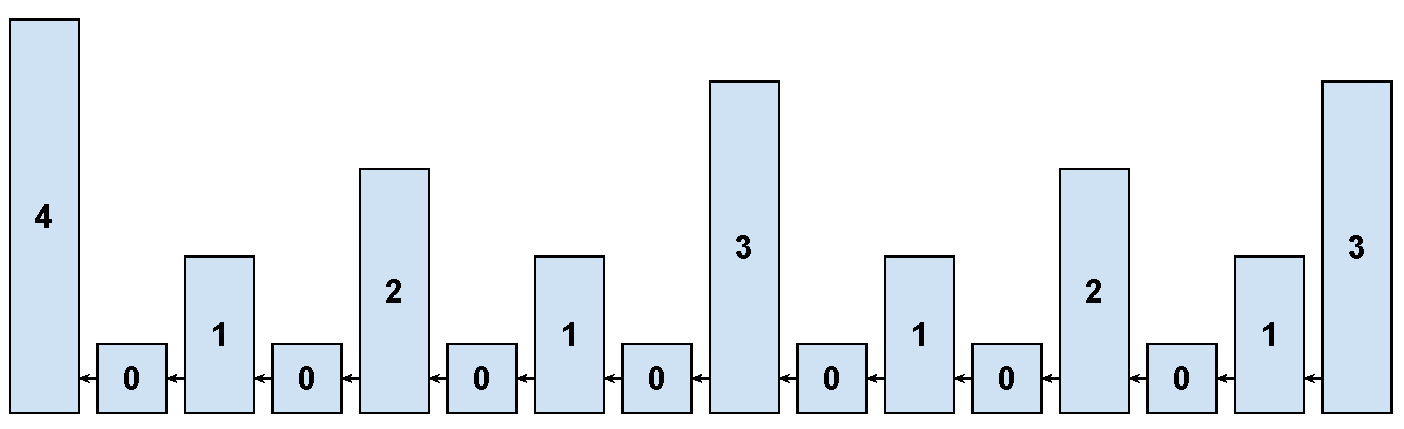
\includegraphics[width=0.7\columnwidth,keepaspectratio]{chapters/work/figures/hierarchical-chain-tall.pdf}
  \label{fig.hierarchy2}
\end{figure}

\subsection*{Αποδείξεις Απόδειξης Εργασίας}

Στο πρόβλημα του συγχρονισμού, ένας τίμιος κόμβος, ο \emph{επαληθευτής}, που θέλει να συγχρονιστεί με το δίκτυο,
συνδέεται με πολλαπλούς άλλους κόμβους, τους \emph{αποδείκτες}, από τους
οποίους τουλάχιστον ένας είναι τίμιος. Στη συνέχεια, στην περίπτωση του SPV, κατεβάζει από εκείνους
υποψήφιες αλυσίδες κεφαλίδων, τις συγκρίνει, και επιλέγει εκείνη με την περισσότερη εργασία. Το
πρόβλημα έγγυται στο να μειώσουμε ασυμπτωτικά την πολυπλοκότητα επικοινωνίας από γραμμική στο χρόνο
εκτέλεσης, όπως είναι στο SPV, σε πολυλογαριθμική. Τα δεδομένα που θα ανταλλάσσονται θα είναι σύντομα
αλφαριθμητικά που αποδεικνύουν ότι \emph{υφίσταται} υποβόσκουσα απόδειξη εργασίας χωρίς να την καταδεικνύουν
αυτούσια. Ως τέτοια, θα τα ονομάζουμε \emph{αποδείξεις απόδειξης εργασίας}. Κεντρική τεχνική συμβολή της
παρούσας διατριβής αποτελεί η κατασκευή τέτοιων αποδείξεων απόδειξης.

Μία πρώτη ιδέα για την κατασκευή αποδείξεων απόδειξης εργασίας είναι η εξής. Καθώς, έχοντας μία αλυσίδα,
μπορούμε να επιχειρηματολογήσουμε ότι τα superblocks μέσα της εμφανίζονται με προβλέψιμες κατανομές,
ακολουθούμε την αντίστροφη συλλογιστική για να επιχειρηματολογήσουμε ότι, αν στο δίκτυο έχει εμφανιστεί
ένας επαρκής αριθμός από superblocks ενός επιθυμητού επιπέδου, μπορούμε να συμπεράνουμε ότι υφίσταται
και μία υποβόσκουσα αλυσίδα ανάλογου μεγέθους. Φερ' ειπείν, η εμφάνιση $m$ superblocks επιπέδου $\mu = 10$
υποδεικνύει την ύπαρξη μίας αλυσίδας μεγέθους $m 2^\mu = 1024m$ χωρίς αυτή να έχει παρουσιαστεί. Ο λόγος είναι ότι
τα $m$ αυτά $\mu$-superblocks έχουν εξορυχθεί μέσα από μία διαδικασία που εξορύσσει $0$-superblocks και,
λόγω τυχαιότητας, μπορεί να επιτύχει μερικές φορές, με πιθανότητα $2^{-\mu}$, ένα έγκυρο block να είναι \emph{και}
$\mu$-superblock. Επιπλέον, ο αντίπαλος δεν μπορεί να αφιερώσει την υπολογιστική του ισχύ στο να παράξει
$\mu$-superblocks γρηγορότερα απ' ό,τι θα μπορούσε να τα παράξει αν επιχειρούσε απλώς την εξόρυξη έγκυρων
blocks, δηλαδή με επαναλαμβανόμενα ερωτήματα στο τυχαίο μαντείο, την συνάρτηση κατακερματισμού. Θα
αφιερώσουμε μεγάλο μέρος της παρούσας διατριβής στο να αποδεικνύουμε με αυστηρότητα θεωρήματα ασφάλειας που δείχνουν
ότι \emph{κανένας} αντίπαλος, ακόμη και αντίπαλοι τους οποίους δεν έχουμε φανταστεί, δεν μπορεί να
ακολουθήσει στρατηγικές που να διαβάλλουν αυτές τις ιδιότητες.

Έτσι, θα μπορούσαμε να σχεδιάσουμε το πρωτόκολλο ως εξής. Αρχικά, ο επαληθευτής επιλέγει μία παράμετρο
ασφάλειας $m \in \mathbb{N}$, το πλήθος των superblocks που θέλει να δει για να πειστεί. Στη συνέχεια,
ο τίμιος αποδείκτης επιλέγει το υψηλότερο επίπεδο $\mu \in \mathbb{N}$ που περιέχει τουλάχιστον $m$
superblocks και τα στέλνει στον επαληθευτή. Σε περίπτωση που όλοι οι αποδείκτες χρησιμοποιήσουν το
ίδιο $\mu$, όταν ο επαληθευτής λάβει διαφορετικό πλήθος $\mu$-superblocks
από τον εκάστοτε αποδείκτη, επιλέγει τον ισχυρισμό εκείνου που του έχει στείλει
τα περισσότερα $\mu$-superblocks και υιοθετεί την αλυσίδα του. Λόγω του τρόπου επιλογής του $\mu$
από τον τίμιο αποδείκτη,
η κατανομή των superblocks μέσα στην αλυσίδα θα είναι τέτοια
ώστε το επίπεδο $\mu$ να περιέχει τουλάχιστον $m$ blocks, ενώ το επίπεδο $\mu + 1$ να περιέχει
λιγότερα από $m$ (αν το επίπεδο $\mu+1$ περιείχε $m$ blocks, τότε το επίπεδο $\mu$ δε θα είχε
επιλεγεί ως μέγιστο από τον τίμιο αποδείκτη). Καθώς το πλήθος των blocks μειώνεται εκθετικά
με ρυθμό $2^{-\mu}$ όσο μεγαλώνει το $\mu$, το πλήθος των blocks μέσα στο επίπεδο $\mu$ θα
είναι κοντά σε $m$. Ο λόγος είναι ότι, αν το πλήθος των blocks ήταν πολύ περισσότερο από $2m$,
τότε θα είχαν εμφανιστεί περίπου\footnote{Στη μαθηματική ανάλυσή μας θα δούμε ότι υπάρχουν επιθέσεις
που καταπνίγουν superblocks υψηλού επιπέδου μέσα σε αλυσίδες χαμηλού επιπέδου μεγάλου μήκους, αλλά
θα ποσοτικοποιήσουμε ακριβώς τον αντίκτυπο που τέτοιες επιθέσεις μπορούν να έχουν.}
$m$ superblocks επιπέδου $\mu+1$ ανάμεσα σε εκείνα, αφού η πιθανότητα
ένα $\mu$-superblock να είναι και $(\mu + 1)$-superblock είναι $\frac{1}{2}$. Έτσι, αν θεωρήσουμε
το $m$ σταθερό, το πρωτόκολλό μας έχει σταθερή πολυπλοκότητα επικοινωνίας.

Ένας τέτοιος επαληθευτής έχει στα χέρια του πλέον ένα σταθερό πλήθος από κεφαλίδες blocks,
ένα δείγμα της υποβόσκουσας αλυσίδας, για το οποίο μπορεί να πάρει αποφάσεις όπως να ελέγξει
τις σποραδικές συναλλαγές που τυχόν έχουν επαληθευτεί εκεί. Θα δούμε ότι, αν ένα τέτοιο δείγμα
είναι σωστό, αυτό επαρκεί για να αποδειχθεί, με σύντομο τρόπο, και η ύπαρξη οποιουδήποτε block
μικρότερου επιπέδου που παρεμβάλλεται ανάμεσα στα $\mu$-superblocks που έχουν παραληφθεί. Έτσι,
οποιαδήποτε συναλλαγή μπορεί να επιβεβαιωθεί με αυτό τον τρόπο.

\subsection*{Η Διασυνδεδεμένη Αλυσίδα}
Για να αποφευχθούν περιστατικά προεξόρυξης, θα πρέπει να υπάρχει κάποια εγγύηση
ότι τα superblocks που ανταλλάσσονται στο πρωτόκολλό μας έχουν εξορυχθεί μετά τη γένεση. Ως εκ τούτου,
ο τίμιος επαληθευτής απαιτεί το πρώτο superblock που θα λάβει να είναι η γένεση. Με αυτό τον τρόπο, η
γένεση θεωρείται εξ' ορισμού ένα superblock που καλύπτει όλα τα επίπεδα.

Ένα πρόβλημα που γίνεται γρήγορα εμφανές με τη συγκεκριμένη δομή είναι ότι ένας αντίπαλος αποδείκτης
μπορεί να αναδιοργανώσει τη σειρά με την οποία εμφανίζονται τα superblocks μέσα σε μία απόδειξη απόδειξης
εργασίας με τρόπο που ο επαληθευτής δεν μπορεί να εντοπίσει. Για παράδειγμα, ένας αντίπαλος αποδείκτης
μπορεί απλώς να παράξει μία τίμια απόδειξη απόδειξης και να στείλει μία μετάθεσή της στον τίμιο επαληθευτή.
Στο απλό μας σχήμα, ο τίμιος επαληθευτής δεν θα μπορέσει να ξεχωρίσει την αντίπαλη απόδειξη από
την τίμια, αφού και οι δύο περιέχουν ακριβώς το ίδιο πλήθος superblocks του επιπέδου
σύγκρισης. Στην πραγματικότητα, η συγκεκριμένη αναδιοργάνωση επιτρέπει σε έναν αντίπαλο να πραγματοποιήσει
προεξόρυξη superblocks, καθώς, παρ' όλο που η γένεση εμφανίζεται πρώτη, δεν υπάρχει κάποια διασύνδεση
κατακερματισμού από το κάθε block πίσω στη γένεση.

Η αιτία του προβλήματος προέρχεται από το ότι, ενώ στα blocks επιπέδου $0$ υπάρχουν δείκτες από κάθε
block στο προηγούμενό του, αντιθέτως, στο $\mu$-οστό επίπεδο κάτι τέτοιο δεν υφίσταται. Για την
θεραπεία αυτού του προβλήματος, λοιπόν, προτείνουμε την προσθήκη δεικτών ανάμεσα στα διαδοχικά
superblocks κάθε επιπέδου. Δηλαδή, θα μας ήταν χρήσιμο κάθε $\mu$-superblock να περιέχει ένα δείκτη
στο πιο πρόσφατο $\mu$-superblock που προηγείται. Για τεχνικούς λόγους, επιλέγουμε να
προσθέσουμε \emph{όλους} τους δείκτες σε \emph{όλα} τα πιο πρόσφατα superblocks κάθε επιπέδου όταν
εξορύσσουμε το κάθε νέο block.
Η πιθανή ανησυχία ότι μία τέτοια δομή θα έχει δυσανάλογα μεγάλο μέγεθος απαντάται παρατηρώντας ότι
το πλήθος των επιπέδων είναι ασυμπτωτικά $\Theta(\log |\chain|)$.
Μία τέτοια διασύνδεση απεικονίζεται στην Εικόνα~\ref{fig.summary-level-shadows}.

\begin{figure}
  \caption{Η διασυνδεδεμένη αλυσίδα. Κάθε superblock περιέχει δείκτες σε όλα τα προηγούμενα superblocks
  του που δεν επισκιάζονται από άλλα.}
  \centering
  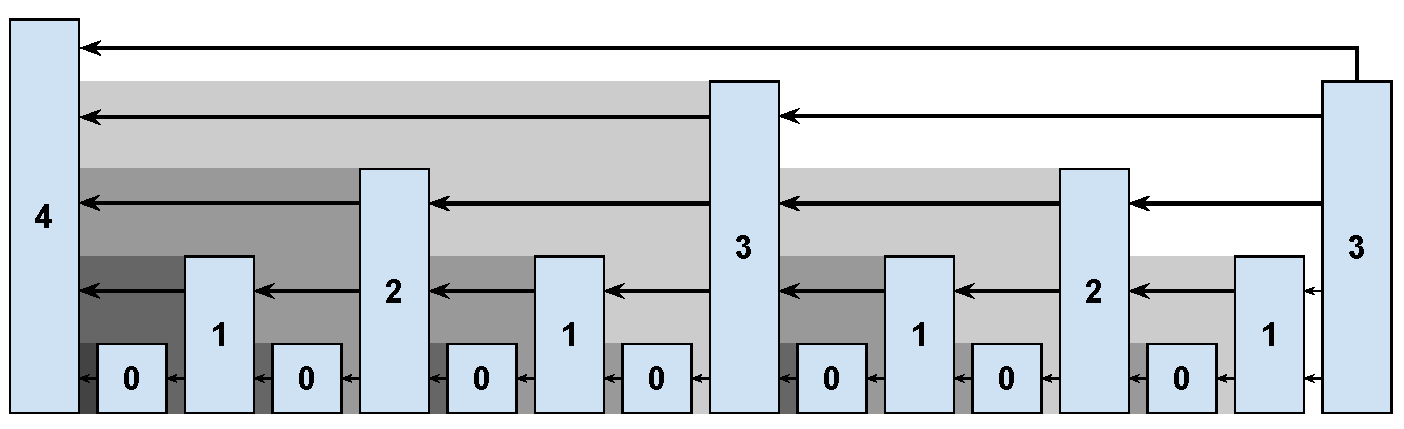
\includegraphics[width=0.7\columnwidth,keepaspectratio]{chapters/work/figures/level-shadows.pdf}
  \label{fig.summary-level-shadows}
\end{figure}

Αυτή η διασύνδεση της αλυσίδας μάς επιτρέπει να μεταβούμε από την ανταλλαγή \emph{συνόλων} superblocks
στην ανταλλαγή \emph{αλυσίδων} superblocks και λύνει το πρόβλημα της αυθαίρετης αναδιάταξης και της
προεξόρυξης.

Η παράμετρος $m$ χρησιμοποιείται από τον επαληθευτή ως \emph{παράμετρος ασφάλειας}: Επιλέγεται έτσι
ώστε η πιθανότητα επιτυχίας ενός αντιπάλου να πέφτει εκθετικά στο $m$. Παρ' όλα αυτά, βλέπουμε ότι
ο αντίπαλος δεν είναι απαραίτητο να έχει παράξει ο ίδιος όλα τα $m$ $\mu$-superblocks που θα στείλει
στην απόδειξή του, αλλά μπορεί να υιοθετήσει και κάποια από τα $\mu$-superblocks που έχουν εξορύξει
τίμιοι. Για παράδειγμα, αν ο τίμιος αποδείκτης
στείλει μία απόδειξη απόδειξης $\pi$ μέγεθους $|\pi| = m$ επιπέδου $\mu$, εύκολα ένας αντίπαλος
μπορεί να παράξει μία νέα απόδειξη απόδειξης $\pi'$ στην οποία θα έχει αντικαταστήσει μόνο το
πιο πρόσφατο $\mu$-superblock από αυτά. Ο αντίπαλος μπορεί να πετύχει μία τέτοια εξόρυξη
με μη αμελητέα πιθανότητα. Ως εκ τούτου, το πρωτόκολλό μας θα πρέπει να ακολουθήσει μία πιο χειρουργική
διαδικασία για να πραγματοποιήσει τη σύγκριση. Το πρωτόκολλο του τίμιου επαληθευτή επιγραμματικά
ακολουθεί τα παρακάτω βήματα. Έχοντας λάβει δύο αποδείξεις αποδείξεων $\pi_A$ και $\pi_B$, ο
επαληθευτής αρχικά εντοπίζει τον πιο πρόσφατο κοινό πρόγονο $b$ ανάμεσα στις δύο αποδείξεις. Στη
συνέχεια, απαιτεί από τους αποδείκτες να στείλουν $m$ superblocks του υψηλότερου επιπέδου που μπορούν
ανάμεσα στα blocks που είναι απόγονοι του $b$ και εμπεριέχονται στις εκάστοτε υποβόσκουσες αλυσίδες τους. Η
διαδικασία αυτή μπορεί να συνεχιστεί επαγωγικά εντοπίζοντας έναν νέο πιο πρόσφατο κοινό πρόγονο $b$,
έως ότου ένας εκ των δύο αποδεικτών να είναι ανύμπορος να ανταπεξέλθει, ή μέχρι η διαδικασία να φτάσει
στη βάση της επαγωγής στο επίπεδο $\mu = 0$ (μπορούμε να δείξουμε ότι αυτά τα δύο γεγονότα είναι
εξαντλητικά με συντριπτική πιθανότητα).

Για να αφαιρέσουμε το κομμάτι της διαδραστικότητας από το παραπάνω πρωτόκολλο, μεταβάλλουμε τον τίμιο
αποδείκτη ως εξής. Ο αποδείκτης συλλλέγει superblocks διαδοχικών επιπέδων τα οποία θα στείλει
στην απόδειξη απόδειξής του, ξεκινώντας από το υψηλότερο επίπεδο και καταλήγοντας στο μηδενικό.
Αρχικά, συμπεριλαμβάνει όλα τα blocks του υψηλότερου επιπέδου $\mu$ που
περιέχει τουλάχιστον $m$ blocks. Στη συνέχεια, αν ο αποδείκτης έχει ήδη αποφανθεί για τα blocks
κάποιου επιπέδου $\mu$, συλλέγει τα blocks του επιπέδου $\mu - 1$ επαγωγικά ως εξής.
Εντοπίζει το $m$-οστό από το τέλος block $b$ ανάμεσα σε όλα τα $\mu$-superblocks που έχει ήδη
συλλέξει και στη συνέχεια συμπεριλαμβάνει όλα τα $(\mu - 1)$-superblocks που έπονται του $b$,
τα οποία θα είναι περίπου $2m$ σε πλήθος. Με λίγα λόγια, ο αποδείκτης θα συμπεριλάβει στην
αναμενόμενη περίπτωση τα $2m$ πιο πρόσφατα blocks κάθε επιπέδου. Όπως θα δούμε στην ανάλυσή μας,
αυτά τα superblocks στις αποδείξεις αποδείξεων, που είναι ασυμπτωτικά μόνο $2m \log|\chain|$ σε πλήθος,
επαρκούν ώστε ο επαληθευτής να ακολουθήσει την παραπάνω κατιούσα επαγωγική διαδικασία σύγκρισης και
να εξάγει το νικητή χωρίς επιπλέον αλληλεπιδράσεις. Έτσι, οι αποδείξεις μας είναι λογαριθμικές στο
μέγεθος της αλυσίδας.

Μέχρι στιγμής έχουμε υποθέσει ότι και οι δύο αποδείκτες θα στείλουν blocks του ίδιου επιπέδου $\mu$.
Όμως ενδέχεται ένας εκ των δύο επαληθευτών να μην μπορεί να στείλει τουλάχιστον $m$ superblocks επιπέδου
$\mu$, αλλά οι δύο επαληθευτές να καταλήξουν σε διαφορετικά επίπεδα $\mu_A$, $\mu_B$ όταν αναζητούν
το επίπεδο της αλυσίδας τους που περιέχει τουλάχιστον $m$ blocks του εν λόγω επιπέδου. Ο επαληθευτής
συνεπώς καλείται να κάνει μία σύγκριση ανάμεσα σε δύο διαφορετικά επίπεδα. Για να γίνει κάτι τέτοιο,
το πλήθος των blocks που έχει στείλει ο κάθε αποδείκτης πρέπει να καταμετρηθεί λαμβάνοντας υπ' όψιν
το βάρος της σπανιότητας του επιπέδου που επιλέγει να στείλει. Έτσι, ο αποδείκτης που λαμβάνει δύο
αποδείξεις $\pi_A$ και $\pi_B$ επιπέδων $\mu_A$ και $\mu_B$ αντίστοιχα θα πρέπει να πραγματοποιήσει
τη σύγκριση ελέγχοντας αν $2^\mu_A |\pi_A| \leq 2^\mu_B |\pi_B|$. Στην παρούσα διατριβή θα παρουσιάσουμε
δύο κατασκευές για σύγκριση αποδείξεων απόδειξης. Στην πρώτη, που ονομάζουμε
\emph{κατασκευή γενναιοδωρίας}, η σύγκριση γίνεται λαμβάνοντας υπόψιν διαφορετικά επίπεδα σε κάθε
απόδειξη απόδειξης και χρησιμοποιώντας αυτά τα βάρη. Στην δεύτερη, που ονομάζουμε
\emph{κατασκευή απόσταξης}, ο τίμιος επαληθευτής επιλέγει ένα κοινό επίπεδο σύγκρισης στο οποίο μπορεί
να συγκρίνει το μέγεθος της εκάστοτε superblock αλυσίδας ως προς απλώς το μέγεθος.

% \subsection*{Απαντώντας σε ερωτήματα}

Χρησιμοποιώντας το πρωτόκολλο αποδείξεων απόδειξης εργασίας που είναι ταυτόχρονα
μη διαδραστικό και έχει λογαριθμική πολυπλοκότητα επικοινωνίας, μπορεί κανείς να
σχεδιάσει υπερελαφρείς κόμβους. Οι αποδείξεις αποδείξεων
που απαιτούνται για να πετύχει κανείς ασφάλεια συγκρίσιμη με πλήρεις κόμβους έχουν
μέγεθος μερικές εκατοντάδες KB στην περίπτωση του Bitcoin σήμερα. Είναι,
συνεπώς, κατάλληλες για συγχρονισμό σε δίκτυα με περιορισμένο εύρος ζώνης και
σε φορητές συσκευές με μικρό αποθηκευτικό χώρο και υπολογιστική ισχύ. Οι επιβεβαίωση
που πρέπει να εκτελέσει το πορτοφόλι που λειτουργεί σαν επαληθευτής δεν αποτελείται από τίποτε
άλλο πέρα από ελέγχους συναρτήσεων κατακερματισμού, κάτι που υλοποιείται αποδοτικά
και σε συσκευές με περιορισμούς.

Οι μέθοδοι υπερελαφρών κόμβων μπορούν να χρησιμοποιηθούν όχι μόνο από πορτοφόλια,
αλλά και από υπερελαφρείς εξορύκτες, οι οποίοι μπορούν πλέον να διατηρούν μόνο λογαριθμικά
δεδομένα στη μνήμη τους.

\subsection*{Γενικεύοντας το Μοντέλο}
Γενικεύουμε το μοντέλο μας χαλαρώνοντας δύο υποθέσεις. Από τη μία την υπόθεση \emph{στατικής
δυσκολίας} και από την άλλη την υπόθεση \emph{συγχρονισμένου δικτύου}.

Στην παραπάνω συζήτηση, παρουσιάσαμε ένα πρωτόκολλο το οποίο λειτουργεί στο μοντέλο
\emph{στατικής δυσκολίας}, όπου δηλαδή ο στόχος απόδειξης εργασίας $T$ είναι σταθερός
σε όλη τη διάρκεια εκτέλεσης του πρωτοκόλλου. Οι πραγματικές αλυσίδες, όμως, ακολουθούν
πρωτόκολλα \emph{δυναμικής δυσκολίας} όπου ο στόχος απόδειξης εργασίας αλλάζει από εποχή
σε εποχή. Αυτό κάνει την ανάλυση ιδιαίτερα περίπλοκη. Το πρωτόκολλό μας, και συγκεκριμένα
η \emph{γενναιόδωρη κατασκευή}, συνεχίζει να δουλεύει στο μοντέλο δυναμικής δυσκολίας,
εφόσον οι παράμετροι του συστήματος παραμένουν εντός λογικών ορίων.
Συγκεκριμένα, η
διάρκεια μίας εποχής πρέπει να είναι αρκετά μεγάλη σε σχέση με την παράμετρο ασφάλειας
$m$.
Αντίστοιχοι περιορισμοί θα πρέπει να εφαρμόζονται και στο πόσο γρήγορα επιτρέπεται να
μεταβληθεί ο πληθυσμός των εξορυκτών σε μικρό χρονικό διάστημα, δηλαδή η δυσκολία δεν
επιτρέπεται να αλλάζει δραματικά.
% Οι περιορισμοί στην αυξομείωση του πληθυσμού πρέπει
% να φράσσονται από την βάση του λογαρίθμου στα επίπεδα των superblocks. Για παράδειγμα,
% όταν δύο διαδοχικά επίπεδα superblocks περιέχουν το ένα διπλάσια superblocks από το ανώτερό του,
% τότε η δυσκολία σε διαδοχικές εποχές απαγορεύεται να αυξομειωθεί περισσότερο από το
% διπλάσιο ή το υποδιπλάσιο. Διαφορετικές βάσεις λογαρίθμου επιτρέπουν διαφορετικές αυξομειώσεις
% δυσκολίας, με τίμημα οι αποδείξεις αποδείξεων να μεγαλώνουν σε μέγεθος όταν η ανεκτικότητα
% γίνεται ελαστική.

Η βασική κατασκευή παραμένει η ίδια, με την διαφορά ότι, πλέον, παρ' όλο που το πρωτόκολλο
έχει μία μεταβαλλόμενη δυσκολία $T_r$ σε κάθε γύρο $r$, οι αποδείξεις αποδείξεων κατασκευάζονται
με γνώμονα την αρχική δυσκολία $T_0$. Αντίστοιχα και ο ορισμός ενός superblock γίνεται έχοντας
ως σημείο αναφοράς την αρχική δυσκολία $T_0$. Έτσι, όταν η δυσκολία της υποβόσκουσας αλυσίδας
αυξηθεί, τα superblocks από ένα επίπεδο και κάτω δεν θα είναι έγκυρα blocks. Το πρωτόκολλο
που παρουσιάστηκε συνοπτικά παραπάνω επιτρέπει στον επαληθευτή να καταλήξει σε μία αλυσίδα
superblocks η οποία έχει μία ενδιαφέρουσα ιδιότητα: Αν αφαιρεθεί από το τέλος της ένα πλήθος
blocks που αντιστοιχεί στην εργασία που αντιπροσωπεύουν $k$ blocks της τελικής δυσκολίας, η
αλυσίδα superblocks που απομένει είναι υποσύνολο όλων των υποβόσκουσων αλυσίδων που έχουν
υιοθετήσει τίμιοι κόμβοι. Συνεπώς, ο επαληθευτής αντιμετωπίζει πλέον μόνο μία πρόκληση:
Ποια blocks να υιοθετήσει ως ευσταθή και ποια να απορρίψει ως ασταθή. Για να κάνει κάτι
τέτοιο, αρκεί να εκτιμήσει την τρέχουσα δυσκολία που εξορύσσει το υπόλοιπο δίκτυο. Με
αυτό το σκοπό, προτείνουμε μία άλλη κατασκευή που ονομάζουμε \emph{μετεωρολογικά μπαλόνια}.
Ένα τέτοιο μπαλόνι είναι μία δειγματοληπτική συναλλαγή που περιέχει υψηλή εντροπία και
εκπέμπει ο επαληθευτής στο δίκτυο. Στη συνέχεια περιμένει για ένα χρονικό διάστημα επαρκούς
διάρκειας για να δει τα blocks τα οποία θα συμπεριλάβουν άμεσα ή έμμεσα αυτή τη συναλλαγή.
Η δυσκολία αυτών των blocks αθροιστικά μπορεί να χρησιμοποιηθεί για να εκτιμήσει κανείς
την τρέχουσα εργασία που παράγει το δίκτυο συνολικά και επιτρέπει στον επαληθευτή να
εξάγει ένα κάτω και ένα άνω φράγμα γι' αυτήν, ανεξαρτήτως της συμπεριφοράς του αντιπάλου.
Οπλισμένος με αυτή την πληροφορία, και επιλέγοντας συντηρητικά τη χειρότερη εκτίμηση που
έχει κάνει όσο αφορά τη δυσκολία του δικτύου, ο επαληθευτής μπορεί πλέον με σιγουριά να
επιλέξει ένα superblock που έχει δύο ιδιότητες. Από τη μία, έχει υιοθετηθεί από όλους τους
τίμιους κόμβους στις εκάστοτε υποβόσκουσες αλυσίδες τους. Από την άλλη, δεν βρίσκεται πολύ
μακριά από το πέρας της αλυσίδας σε καμία από αυτές. Το μέγεθος που χρειάζεται να κατεβάσει
από το δίκτυο ο τίμιος κόμβος για να συμπληρώσει το τελευταίο κομμάτι της αλυσίδας που
απομένει είναι σταθερό και δεν συμβάλλει στην πολυπλοκότητα του πρωτοκόλλου.

Όσο αφορά το μοντέλο συγχρονισμένου δικτύου, η παραπάνω ανάλυση υποθέτει ότι τα μηνύματα που
εκπέμπουν οι τίμιοι κόμβοι στο δίκτυο φτάνουν στους ομότιμούς τους μέσα σε ένα γύρο.
Χαλαρώνουμε την παραπάνω υπόθεση εργαζόμενοι στο $\Delta$-φραγμένο μοντέλο όπου τα μηνύματα
μπορούν να καθυστερήσουν έως $\Delta$ γύρους, αλλά το $\Delta$ δεν είναι γνωστό στους τίμιους
κόμβους, παρ' όλο που υπάγεται σε ορισμένους περιορισμούς εκφρασμένους στη μορφή κατηγορημάτων
που έχει ορίσει ο σχεδιαστής. Στο συγκεκριμένο μοντέλο, ο αντίπαλος έχει ένα πλεονέκτημα $\Delta$
γύρων έναντι των τίμιων παικτών, κάτι που δυσχεραίνει την λειτουργία τους. Συγκεκριμένα, για να
μπορέσουν οι τίμιοι να λειτουργήσουν σε αυτό το μοντέλο, θα πρέπει ο αντίπαλος να φράσσεται
στο $1/4$ του συνολικού δικτύου όσο αφορά την υπολογιστική του ισχύ.

\subsection*{Αποδείξεις Αποδείξεων Μεριδίου}
Οι αποδείξεις αποδείξεων εργασίας αποτελούν μία λύση για το πρόβλημα του συγχρονισμού σε
αλυσίδες απόδειξης εργασίας. Για αλυσίδες απόδειξης μεριδίου, το εν λόγω πρωτόκολλο δεν λειτουργεί.
Ο λόγος είναι ότι ο αντίπαλος μπορεί να παράξει όσα ``superblocks'' μεριδίου θέλει και,
αντίθετα από την περίπτωση της απόδειξης εργασίας, το πλήθος των αποδεκτών superblocks
που μπορεί να παράξει δεν αντιστοιχεί στο μέρος του μεριδίου που κατέχει. Τα πράγματα γίνονται
χειρότερα αν αναλογιστούμε ότι η κατανομή μεριδίου εξελίσσεται με το χρόνο και είναι αδύνατο
ένας επαληθευτής που κρατά στα χέρια του μόνο τη γένεση να γνωρίζει την τρέχουσα κατανομή μεριδίου.
Για να την μάθει, όμως, θα πρέπει να ανατρέξει στην αλυσίδα.

Ξεπερνάμε αυτό το πρόβλημα με ένα σχήμα υπογραφών που συμπιέζουν την αλυσίδα απόδειξης μεριδίου
με τρόπο ο οποίος δίνει σημαντικό πλεονέκτημα. Αντίθετα από τις αποδείξεις απόδειξης
εργασίας, το πλεονέκτημα είναι σταθερό και όχι εκθετικό διότι ο τίμιος επαληθευτής θα πρέπει
να ακολουθήσει όλες τις εξελίξεις που έχουν γίνει στην ιδιοκτησία μεριδίων. Η κατασκευή εν
συντομία απαιτεί από τους τίμιους εξορύκτες να παράγουν μία συναλλαγή ανά εποχή η οποία να πιστοποιεί
την εξέλιξη μεριδίου. Η συμβολή μας εδώ αποτελείται από ένα σχήμα υπογραφής που επιτρέπει σε όλους
τους μεριδιακούς αντιπροσώπους να συνενώσουν τόσο τα κλειδιά τους όσο και τις υπογραφές σε
ένα συνοπτικό κλειδί και μία συνοπτική υπογραφή αντίστοιχα, χωρίς να απαιτείται διαδραστικότητα
μεταξύ τους. Έτσι, ο επαληθευτής αρκεί να ελέγξει μία υπογραφή ανά εποχή για να καταλήξει
στην τρέχουσα κατανομή μεριδίων, μία επιτροπή αντιπροσώπων εκ της οποίας στη συνέχεια μπορεί να τον ενημερώσει με έμπιστο
τρόπο για το ποια είναι η κατανομή του χρήματος ή της γενικότερης κατάστασης της αλυσίδας που
επιθυμεί.

\subsection*{Ο Δρόμος προς τη Διαλειτουργικότητα}
Οι κατασκευές αποδείξεων απόδειξης είναι χρήσιμες για το πρόβλημα του συγχρονισμού, αλλά έχουν
μερικές ακόμη πιο ενδιαφέρουσες εφαρμογές. Μία από αυτές είναι η \emph{διαλειτουργικότητα αλυσίδων}.

Κάθε κρυπτονόμισμα σήμερα αποτελεί ένα ανεξάρτητο και μεμονωμένο σύστημα που δεν μπορεί να
επικοινωνήσει με τα υπόλοιπα χωρίς την εγγύηση έμπιστων τρίτων αρχών. Εφαρμογές που απαιτούν
διαλειτουργικότητα σχετίζονται με οποιαδήποτε ανταλλαγή πληροφορίας ανάμεσα σε διαφορετικές αλυσίδες.
Παραδείγματα αποτελούν η μεταφορά χρήματος από μία αλυσίδα σε μία άλλη, ή η συγγραφή ενός έξυπνου
συμβολαίου σε μία αλυσίδα το οποίο εξαρτάται από την κατάσταση μίας άλλης αλυσίδας.
Μέσω των πρωτοκόλλων μας καθιστούμε εφικτή τη διαλειτουργικότητα αλυσίδων.

Ας αναφέρουμε ένα παράδειγμα
κατά το οποίο ένα νόμισμα ακολουθεί μία πορεία περνώντας από μία αλυσίδα σε μία άλλη. Αρχικά ένα
ημεδαπό νόμισμα Α κάποιας ονομαστικής αξίας και ιδιοκτήτη βρίσκεται στην αλυσίδα Α όπου εξορύχθηκε. Ο
ιδιοκτήτης του αρχικά κλειδώνει αυτή την αξία έτσι ώστε να μην μπορεί να μετακινηθεί περαιτέρω.
Το κλείδωμα αυτό περιλαμβάνεται σε μία συναλλαγή η οποία επιβεβαιώνεται στην αλυσίδα Α. Μόλις
το κλείδωμα επιβεβαιωθεί, παράγονται στην αλυσίδα Β νομίσματα τύπου Α της ίδιας αξίας, που πλέον
όμως δεν είναι ημεδαπά. Αυτά τα νομίσματα μπορούν να ανταλλαχθούν ελεύθερα σαν να ήταν ημεδαπά
νομίσματα της αλυσίδας Β, αλλά διατηρούν τη φύση τους ως νομίσματα τύπου Α. Για παράδειγμα, μπορούν
να διασπαστούν όσο αφορά την αξία τους, αλλά και να αλλάξουν ιδιοκτήτες. Οποτεδήποτε κάποιος ιδιοκτήτης
των νομισμάτων τύπου Α στην αλυσίδα Β επιθυμεί, μπορεί να τα καταστρέψει. Η καταστροφή αυτή, που
έχει τη μορφή καψίματος χρήματος, καταγράφεται σε μία συναλλαγή στην αλυσίδα Β η οποία και επιβεβαιώνεται.
Μόλις επιβεβαιωθεί, το αντίστοιχο ποσό απελευθερώνεται από την προηγουμένως κλειδωμένη ποσότητα
που διατηρείται στην αλυσίδα Α. Μία τέτοια μεταφορά χρήματος από αλυσίδα σε αλυσίδα έχει πολλά
πλεονεκτήματα, διότι επιτρέπει ένα νόμισμα τύπου Α να απολαμβάνει τις αρετές της αλυσίδας Β
(όπως ταχύτητα, ευχρηστία, ή χαρακτηριστικά έξυπνων συμβολαίων που μπορεί να μην υπάρχουν στην
αλυσίδα Α) χωρίς να χάνει τη φύση του και χωρίς να είναι απαραίτητο να ανταλλαχθεί για νομίσματα
τύπου Β, κάτι που θα απαιτούσε την ύπαρξη αντισυμβαλλομένων αλλά και θα υπέβαλλε το χρήστη
στο, συχνά τεράστιο, ρίσκο συναλλάγματος.

Ο τρόπος με τον οποίο υλοποιείται το παραπάνω σενάριο έχει ως εξής. Από ένα έξυπνο συμβόλαιο ζει
σε κάθε μία εκ των δύο αλυσίδων. Τα έξυπνα συμβόλαια γνωρίζουν το ένα για το άλλο, έχοντας το
καθένα καταγράψει την διεύθυνση όπου ζει το ομόλογο συμβόλαιό του κατά την εκκίνηση της λειτουργίας
τους. Όταν στέλνονται χρήματα στο συμβόλαιο που ζει στην αλυσίδα Α, τα χρήματα αυτά κρατώνται
από το συμβόλαιο το οποίο λειτουργεί σαν εγγυητής. Η συναλλαγή που παραδίδει τα χρήματα για να
κλειδωθούν στο συμβόλαιο Α επιβεβαιώνεται στην αλυσίδα Α είτε μέσω εργασίας, είτε μέσω μεριδίου.
Ο κόμβος που κατέθεσε τα χρήματα παράγει μία απόδειξη απόδειξης για το κλείδωμα των χρημάτων
του και μεταδίδει αυτή την απόδειξη απόδειξης στο συμβόλαιο που ζει στην αλυσίδα Β καλώντας
μία μέθοδό του που είναι υπεύθυνη για το κόψιμο νέου χρήματος. Παρατηρούμε εδώ ότι η απόδειξη
απόδειξης δεν είναι τίποτε άλλο παρά ένα απλό αλφαριθμητικό και δεν απαιτεί πρόσβαση στο δίκτυο
για την επιβεβαίωσή της. Το έξυπνο συμβόλαιο της αλυσίδας Β στη συνέχεια εκτελεί τα χρέη του
επαληθευτή, ο οποίος υλοποιείται απευθείας εντός του έξυπνου συμβολαίου, λόγου χάρη χρησιμοποιώντας
Solidity. Το συμβόλαιο αναμένει μία προκαθορισμένη χρονική περίοδο σε περίπτωση που η απόδειξη
απόδειξης ήταν κακόβουλη και κάποιος τίμιος προβάλλει αντιρρήσεις. Αν δεν υπάρξουν αντιρρήσεις,
το συμβόλαιο κόβει ισάριθμα νομίσματα τύπου Α εντός της αλυσίδας Β και ορίζει ως ιδιοκτήτη τους
τον κόμβο που τα κλείδωσε στην αλυσίδα A. Τα νομίσματα αυτά μπορούν να αντιπροσωπευθούν με
τη μορφή κερμάτων ERC-20 και να ανταλλαχθούν κατά τα γνωστά. Όταν ο νέος τους ιδιοκτήτης είναι
έτοιμος να τα επιστρέψει στην αλυσίδα Α, τα παραδίδει σε ειδική μέθοδο του συμβολαίου Β το οποίο
τα καίει. Η πράξη καψίματος περιλαμβάνεται σε μία συναλλαγή η οποία επιβεβαιώνεται στην
αλυσίδα Β. Τέλος, μία απόδειξη απόδειξης χρησιμοποιείται με τον ίδιο ακριβώς τρόπο για να
ξεκλειδωθούν τα χρήματα από το έξυπνο συμβόλαιο που κρατά δεσμευμένα τα χρήματα στην αλυσίδα Α.

Συνοπτικά, η συμβολή μας εισάγει την έννοια των μη διαδραστικών αποδείξεων απόδειξης
εργασίας και μεριδίου στο μοντέλο δυναμικής δυσκολίας και $\Delta$-φραγμένου δικτύου.
Τις αξιοποιούμε για να κατασκευάσουμε υπερελαφρείς κόμβους πορτοφολιών
και εξορυκτών, αλλά και για να επιτρέψουμε τη διάδραση έξυπνων συμβολαίων ανάμεσα σε αλυσίδες
εργασίας και μεριδίου.
\clearpage
\fi
